\documentclass[tikz,14pt,fleqn]{article}

% Math
\usepackage[fleqn]{amsmath}
\usepackage{amssymb}
\usepackage{dsfont}
\usepackage{float}

% Insert dummy text
\usepackage{lipsum}  
% Allows to use caption*
\usepackage{caption}
% Scalabale subfigures
\usepackage{subcaption} 
% Code syntax highlighting
\usepackage{minted}
% Hyperlinks
\usepackage{hyperref}
% Customize page layout
\usepackage{geometry}
\geometry{a4paper, margin=1in}
% Page headers and footers
\usepackage{fancyhdr}
\pagestyle{fancy}
\fancyhf{}
\setlength{\parindent}{0pt}
\setlength{\parskip}{0.5\baselineskip}%

% includegraphics
\usepackage{graphicx}




\newcommand{\bmat}[1]{
   \ensuremath{
   \begin{bmatrix}
       #1
   \end{bmatrix}
}}




\usepackage[utf8]{inputenc}


%%%%%%%%%%%%%%%%%%%%%%%%%%%%
%% VARIABLES
\newcommand\namesurname{Albert Cerfeda}
\newcommand\assignment{Assignment 4 - Color and Multi-scale Representations}

\newcommand\subject{Image \& Video Processing}
\newcommand\documentdate{29 May 2023}

% Title content
%%%%%%%%%%%%%%%%%%%%%%%%%%%%
\rhead{\assignment}
\lhead{\namesurname}
%%%%%%%%%%%%%%%%%%%%%%%%%%%%

\rfoot{Page \thepage}


\begin{document}

\begin{titlepage}
   \begin{center}
       \vspace*{0.2cm}

       \textbf{\Large{\subject}}

       \vspace{0.5cm}
        \textbf{\assignment}\\[5mm]
        
            
       \vspace{0.4cm}

        \namesurname
        \begin{figure}[H]
            \centering
        \end{figure}
       \tableofcontents

       \vspace*{\fill}
     
        
\includegraphics[width=0.4\textwidth]{fig/logo.png}
       
        \documentdate \\
        Università della Svizzera italiana\\
        Faculty of Informatics\\
        Switzerland\\

   \end{center}
\end{titlepage}

\section{Color Palette Extraction from Images [7 points]}
\subsection{Linear RGB and sRGB Color Palettes}
In this exercise we are tasked in obtaining the \verb|sRGB| color space by linearizing the \verb|RGB| color space and extracting a color palette from an image. The color palette is then extracted from both color spaces. 
\begin{figure}[h!]
    \vspace*{-0.2cm}
    \inputminted[firstline=134, lastline=145, frame=lines, framesep=2mm, fontsize=\small ]{matlab}{../src/ex1.m}
    \vspace*{-0.5cm}
    \caption{Matlab function converting RGB to the sRGB color space}
    \label{fig:1.1.linearize_code}
\end{figure}\\
\begin{figure}[h!]
    \vspace*{-0.2cm}
    \inputminted[firstline=161, frame=lines, framesep=2mm, fontsize=\small ]{matlab}{../src/ex1.m}
    \vspace*{-0.5cm}
    \caption{Matlab function performing color quantization}
    \label{fig:1.1.quantization_code}
\end{figure}\\
We perform \textit{k-means} clustering\footnote{K-means clustering: \exthref{https://en.wikipedia.org/wiki/K-means_clustering}{en.wikipedia.org}} on the image colors, by treating each pixel color value as a 3-dimensional point and by letting the algorithm find the $k=7$ centroids to cluster similar colors together. The centroids are then used as the color palette. The code is shown in \autoref{fig:1.1.quantization_code}.\\
Results are shown in \autoref{fig:1.1.rgb_palette_layers} and \autoref{fig:1.1.srgb_palette_layers}.

\begin{figure}[h!]
    \centering
    \begin{subfigure}[]{\linewidth}
        \centering
        
\includegraphics[width=0.13\linewidth]{fig/out/1.1.rgb_palette_1.png}
        
\includegraphics[width=0.13\linewidth]{fig/out/1.1.rgb_palette_2.png}
        
\includegraphics[width=0.13\linewidth]{fig/out/1.1.rgb_palette_3.png}
        
\includegraphics[width=0.13\linewidth]{fig/out/1.1.rgb_palette_4.png}
        
\includegraphics[width=0.13\linewidth]{fig/out/1.1.rgb_palette_5.png}
        
\includegraphics[width=0.13\linewidth]{fig/out/1.1.rgb_palette_6.png}
        
\includegraphics[width=0.13\linewidth]{fig/out/1.1.rgb_palette_7.png}\\
        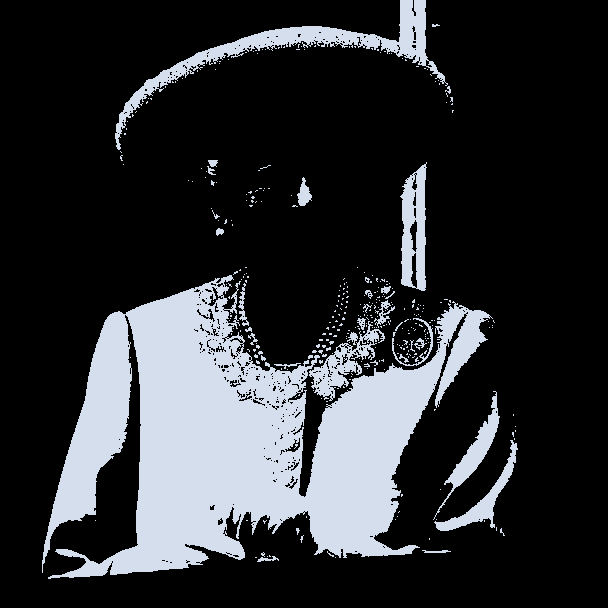
\includegraphics[width=0.13\linewidth]{fig/out/1.1.rgb_layer_1.png}
        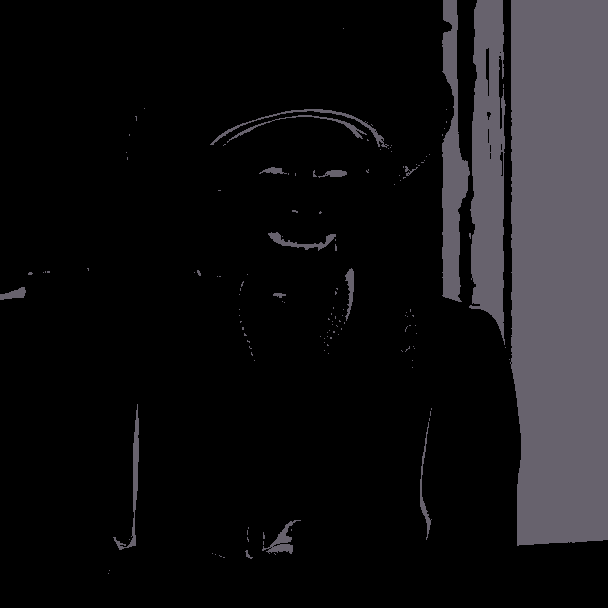
\includegraphics[width=0.13\linewidth]{fig/out/1.1.rgb_layer_2.png}
        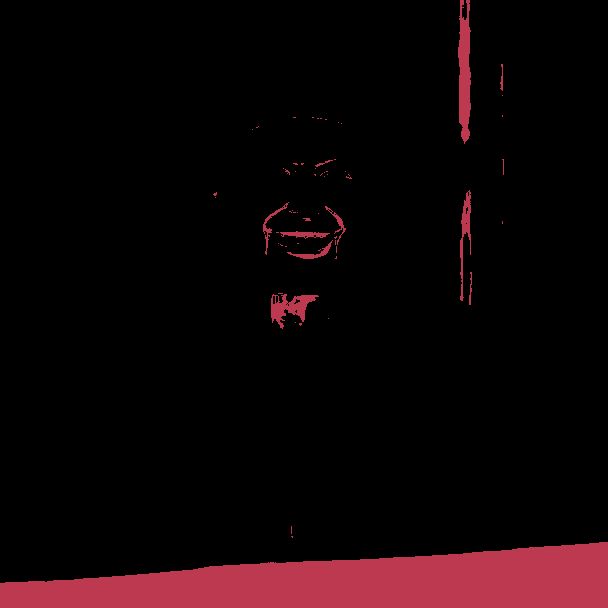
\includegraphics[width=0.13\linewidth]{fig/out/1.1.rgb_layer_3.png}
        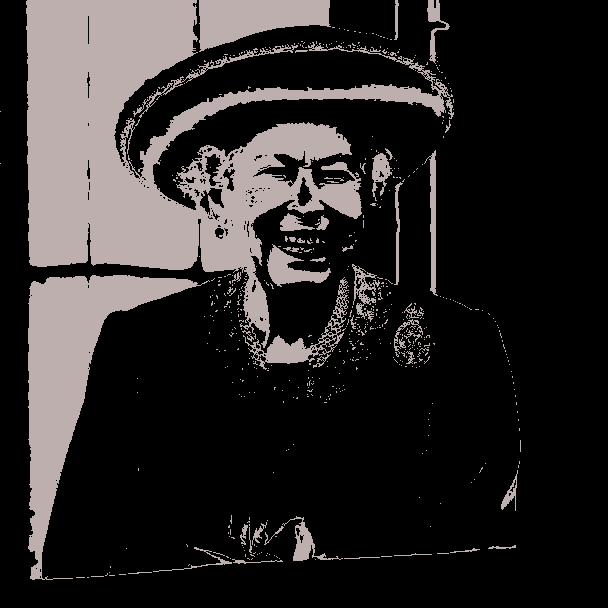
\includegraphics[width=0.13\linewidth]{fig/out/1.1.rgb_layer_4.png}
        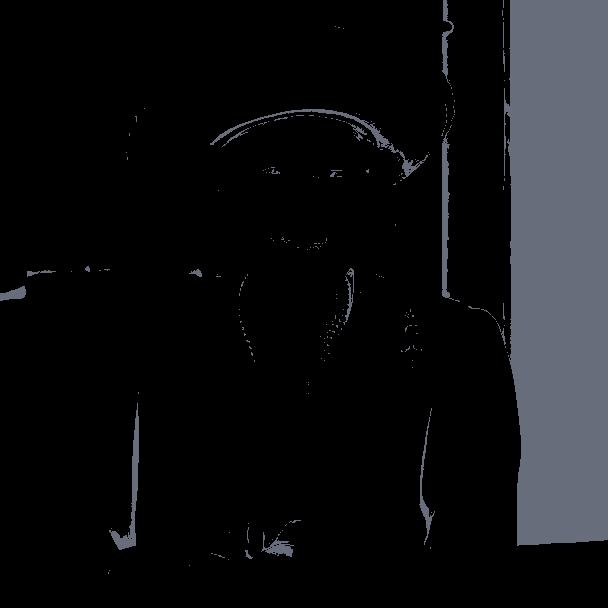
\includegraphics[width=0.13\linewidth]{fig/out/1.1.rgb_layer_5.png}
        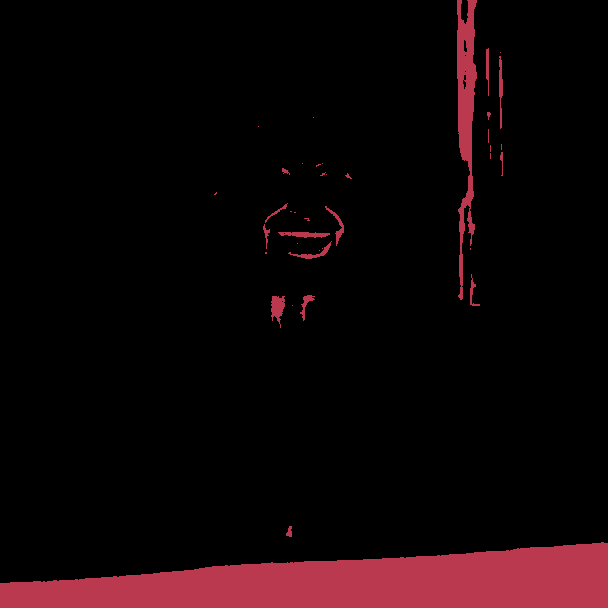
\includegraphics[width=0.13\linewidth]{fig/out/1.1.rgb_layer_6.png}
        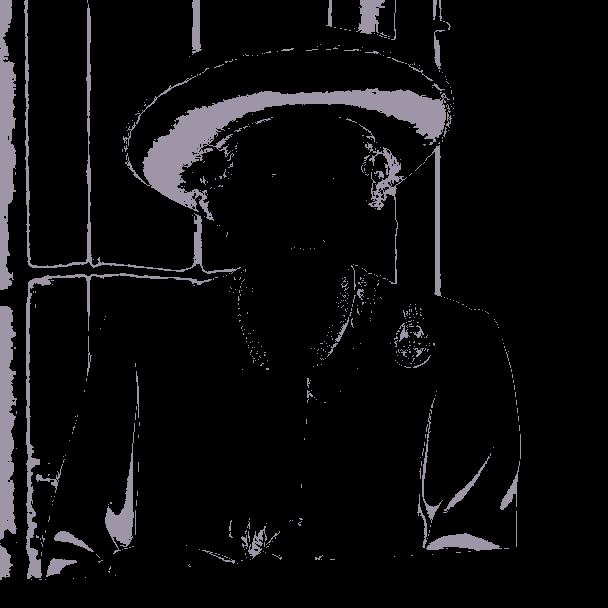
\includegraphics[width=0.13\linewidth]{fig/out/1.1.rgb_layer_7.png}
        \caption{RGB Palette and Layers}
        \label{fig:1.1.rgb_palette_layers}
    \end{subfigure}
    \begin{subfigure}[]{\linewidth}
        \centering
        
\includegraphics[width=0.13\linewidth]{fig/out/1.1.xyz_palette_1.png}
        
\includegraphics[width=0.13\linewidth]{fig/out/1.1.xyz_palette_2.png}
        
\includegraphics[width=0.13\linewidth]{fig/out/1.1.xyz_palette_3.png}
        
\includegraphics[width=0.13\linewidth]{fig/out/1.1.xyz_palette_4.png}
        
\includegraphics[width=0.13\linewidth]{fig/out/1.1.xyz_palette_5.png}
        
\includegraphics[width=0.13\linewidth]{fig/out/1.1.xyz_palette_6.png}
        
\includegraphics[width=0.13\linewidth]{fig/out/1.1.xyz_palette_7.png}\\
        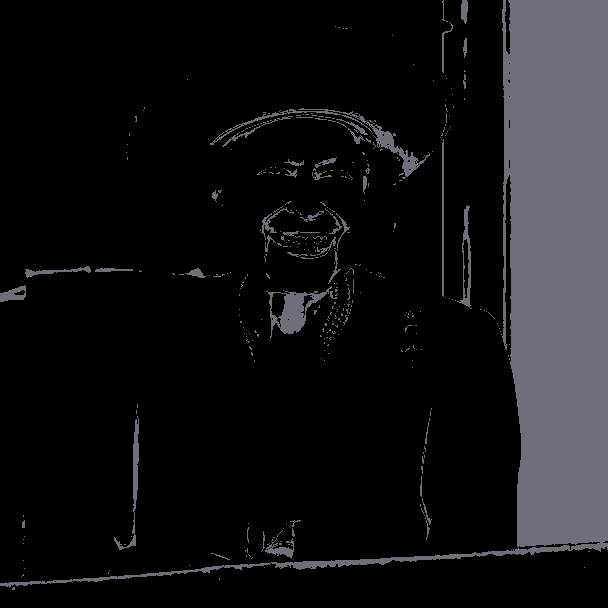
\includegraphics[width=0.13\linewidth]{fig/out/1.1.xyz_layer_1.png}
        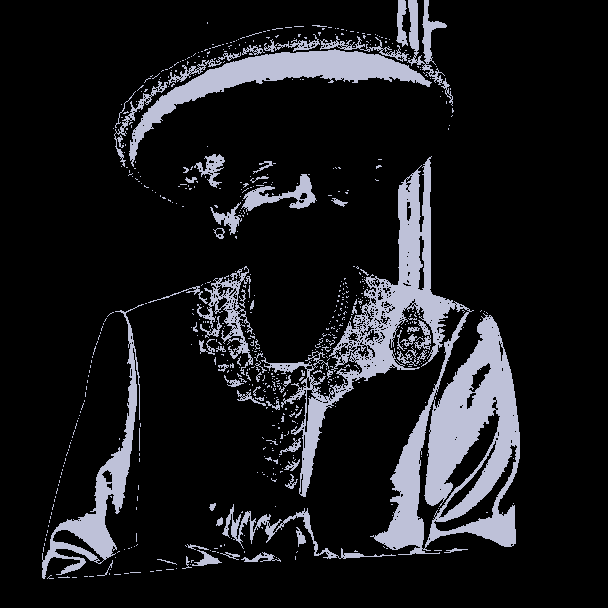
\includegraphics[width=0.13\linewidth]{fig/out/1.1.xyz_layer_2.png}
        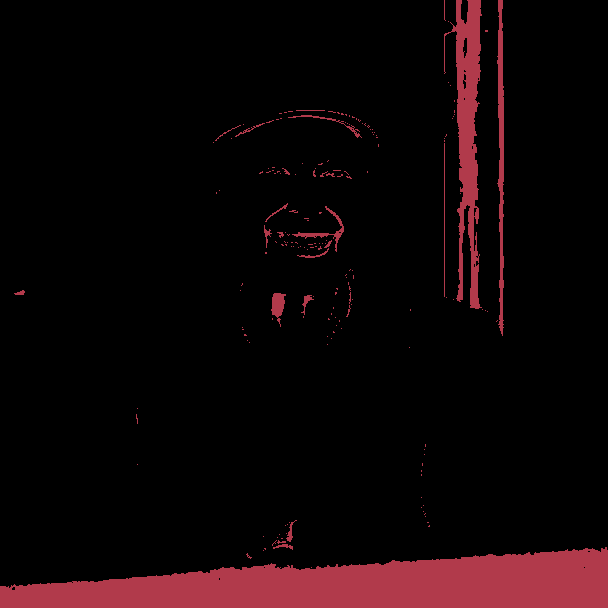
\includegraphics[width=0.13\linewidth]{fig/out/1.1.xyz_layer_3.png}
        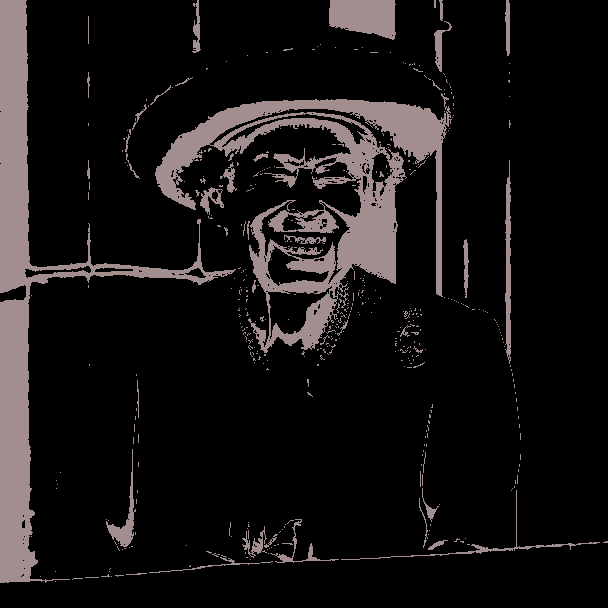
\includegraphics[width=0.13\linewidth]{fig/out/1.1.xyz_layer_4.png}
        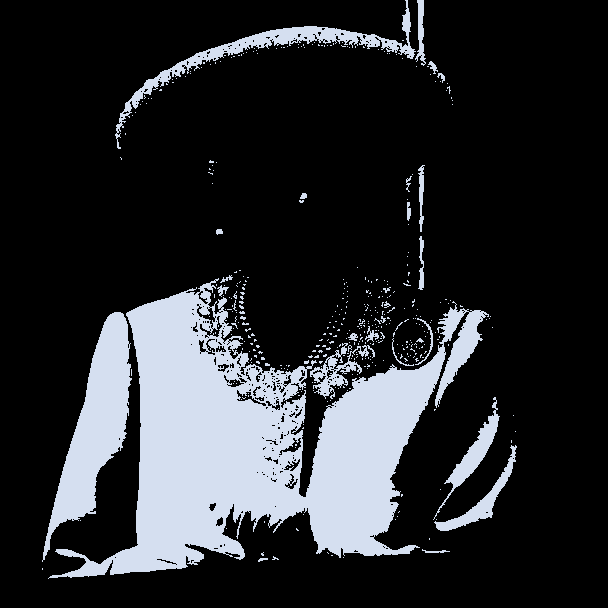
\includegraphics[width=0.13\linewidth]{fig/out/1.1.xyz_layer_5.png}
        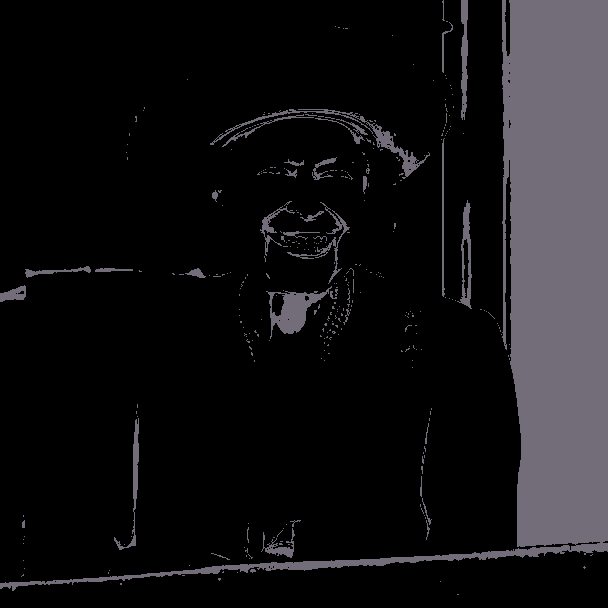
\includegraphics[width=0.13\linewidth]{fig/out/1.1.xyz_layer_6.png}
        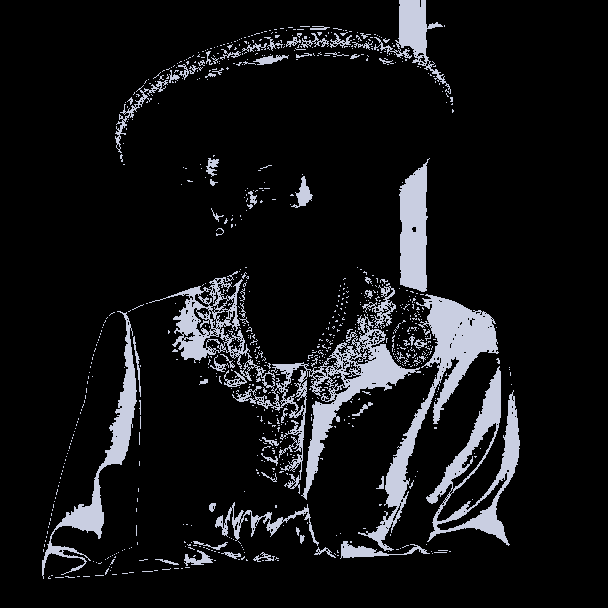
\includegraphics[width=0.13\linewidth]{fig/out/1.1.xyz_layer_7.png}
        \caption{sRGB Palette and Layers}
        \label{fig:1.1.srgb_palette_layers}
    \end{subfigure}

    \begin{subfigure}[]{\linewidth}
        \centering
        
\includegraphics[width=0.13\linewidth]{fig/out/1.2.lab_palette_1.png}
        
\includegraphics[width=0.13\linewidth]{fig/out/1.2.lab_palette_2.png}
        
\includegraphics[width=0.13\linewidth]{fig/out/1.2.lab_palette_3.png}
        
\includegraphics[width=0.13\linewidth]{fig/out/1.2.lab_palette_4.png}
        
\includegraphics[width=0.13\linewidth]{fig/out/1.2.lab_palette_5.png}
        
\includegraphics[width=0.13\linewidth]{fig/out/1.2.lab_palette_6.png}
        
\includegraphics[width=0.13\linewidth]{fig/out/1.2.lab_palette_7.png}\\
        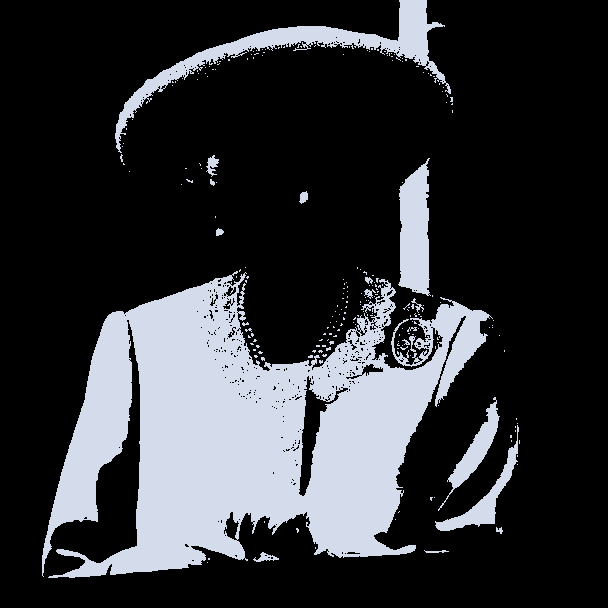
\includegraphics[width=0.13\linewidth]{fig/out/1.2.lab_layer_1.png}
        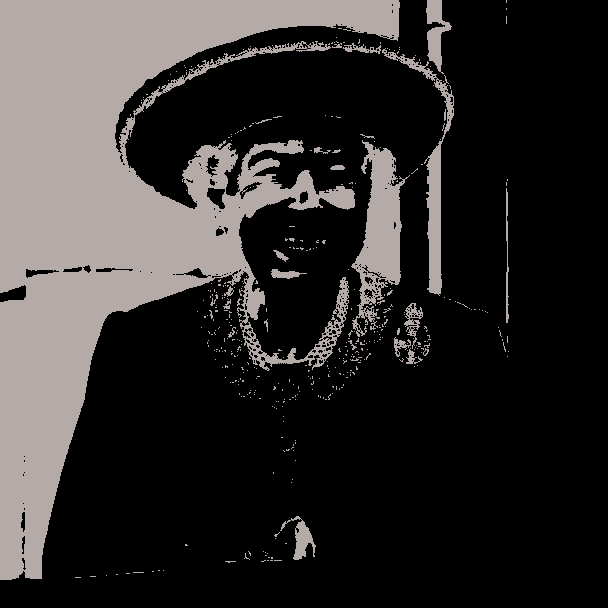
\includegraphics[width=0.13\linewidth]{fig/out/1.2.lab_layer_2.png}
        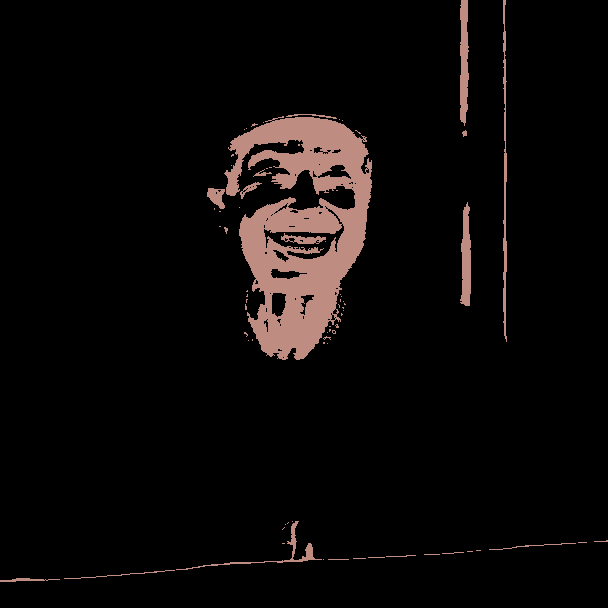
\includegraphics[width=0.13\linewidth]{fig/out/1.2.lab_layer_3.png}
        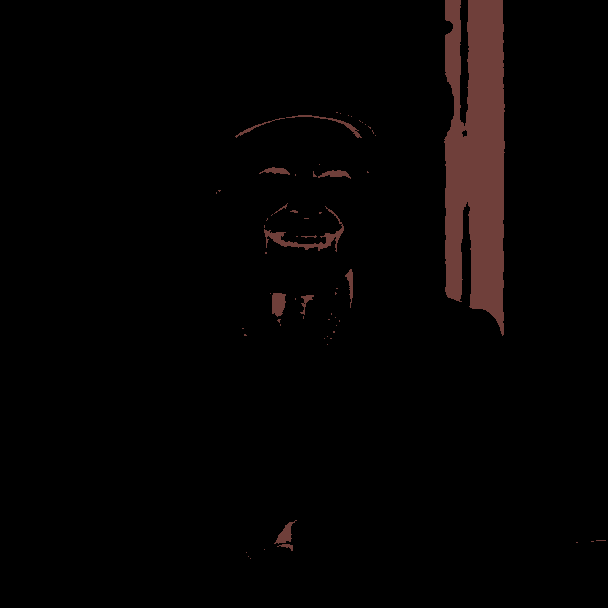
\includegraphics[width=0.13\linewidth]{fig/out/1.2.lab_layer_4.png}
        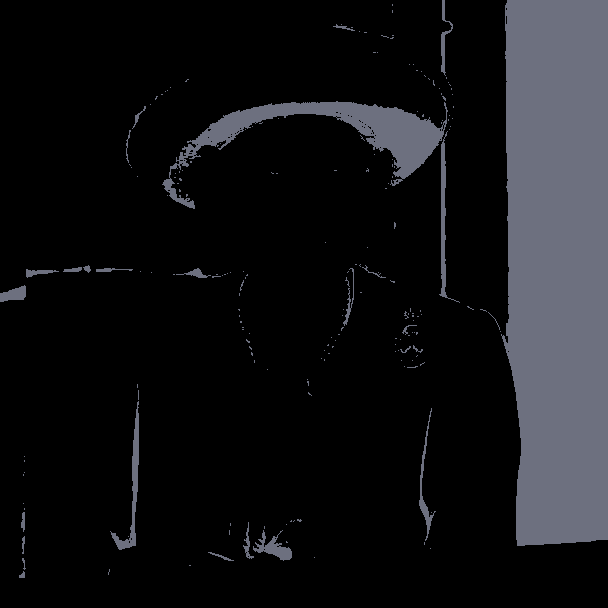
\includegraphics[width=0.13\linewidth]{fig/out/1.2.lab_layer_5.png}
        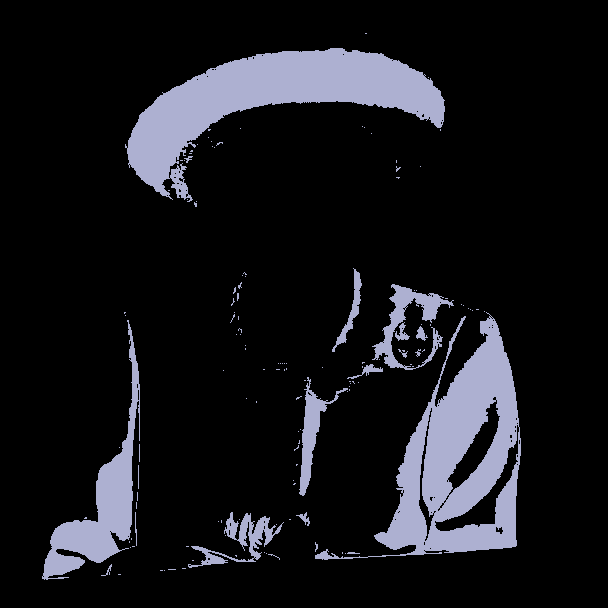
\includegraphics[width=0.13\linewidth]{fig/out/1.2.lab_layer_6.png}
        
\includegraphics[width=0.13\linewidth]{fig/out/1.2.lab_layer_7.png}
        \caption{CIELab Palette and Layers}
        \label{fig:1.2.cielab_palette_layers}
    \end{subfigure}
    \begin{subfigure}[]{0.25\linewidth}
        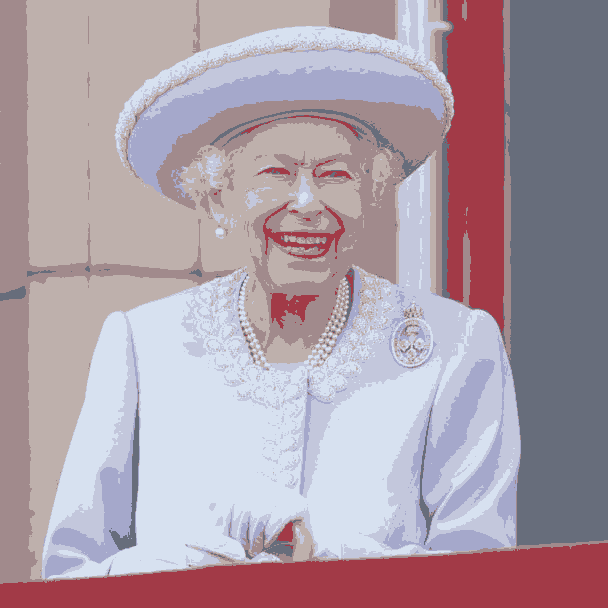
\includegraphics[width=\linewidth]{fig/out/1.1.rgb_clustered.png}
        \caption{RGB Clustered image}
        \label{fig:1.1.rgb_clustered}
    \end{subfigure}
    \begin{subfigure}[]{0.25\linewidth}
        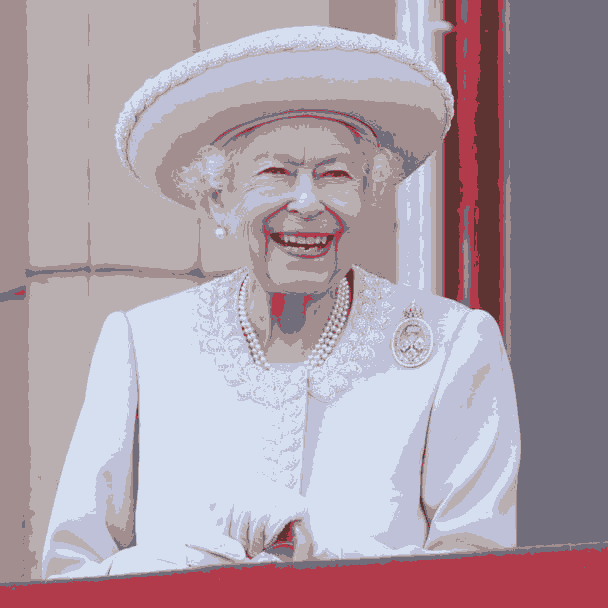
\includegraphics[width=\linewidth]{fig/out/1.1.xyz_clustered.png}
        \caption{sRGB Clustered image}
        \label{fig:1.1.srgb_clustered}
    \end{subfigure}
    \begin{subfigure}[]{0.25\linewidth}
        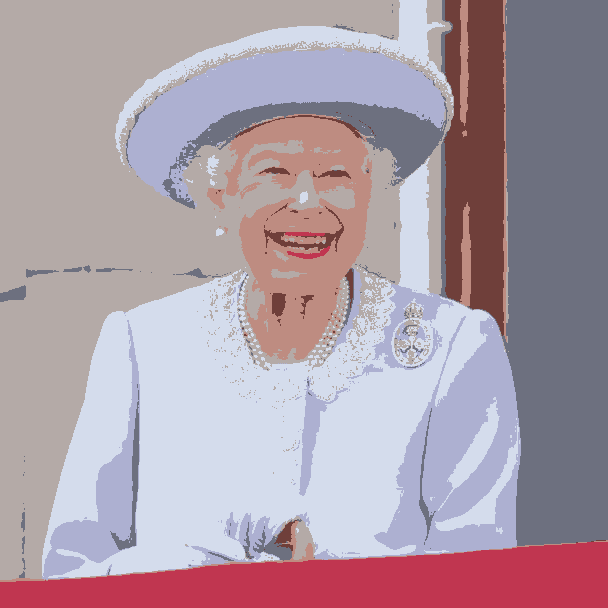
\includegraphics[width=\linewidth]{fig/out/1.2.lab_clustered.png}
        \caption{CIELab Clustered image}
        \label{fig:1.2.cielab_clustered}
    \end{subfigure}
    \caption{Color palette extraction using the RGB, sRGB and CIELab color spaces.}
\end{figure}


\subsection{CIELab Color Palette}
RGB is not the best color model for image processing as, since it specifies the quantities of each Red/Blue/Green pigment for obtaining a color, it not provide us with an intuitive way of understanding and performing operations on colors. For example, it is not straightforward to manipulate the saturation or the brightness of a color in RGB space. An alternative to the RGB color space is the HSV\footnote{HSV: \exthref{https://programmingdesignsystems.com/color/color-models-and-color-spaces/index.html}{programmingdesignsystems.com}} color space. It defines each color using 3 channels: Hue, Saturation and Value, allowing intuitive color manipulations. However, the HSV color space is not perceptually uniform, meaning that the distance between two colors in the HSV space does not correspond to the perceived difference between the two colors.

This is where the CIELab\footnote{CIELab: \exthref{https://www.hunterlab.com/blog/what-is-cielab-color-space/}{hunterlab.com}} comes in handy. The CIELab color space is a perceptually uniform color space, meaning that the distance between two colors in the CIELab space corresponds to the perceived difference between the two color by the human visual system. The CIELab color space is defined by three channels: L*, a* and b*. They represent the lightness of the color (L* = 0 yields black and L* = 100 indicates white), its position between magenta and green (a*, where negative values indicate green and positive values indicate red) and its position between yellow and blue (b*, where negative values indicate blue and positive values indicate yellow).

By clustering colors in the CIELab color space, we will obtain clusters whose points are close to each other in the CIELab space, meaning that they are close to each other in the perceptual space (i.e our eyes perceive these colors as similar), resulting in a better color palette than the one obtained by clustering colors in the RGB space.

% TODO: Finish answering and do Bonus

The artistic look of the clustered image can be modified by changing the color layers individually. In \autoref{fig:1.2.edited} we present the result obtained by altering the hue, saturation and value of various color layers. The result is a colorful image resembling Shrek.

\begin{figure}[H]
    \centering
    \begin{subfigure}[]{0.3\linewidth}
        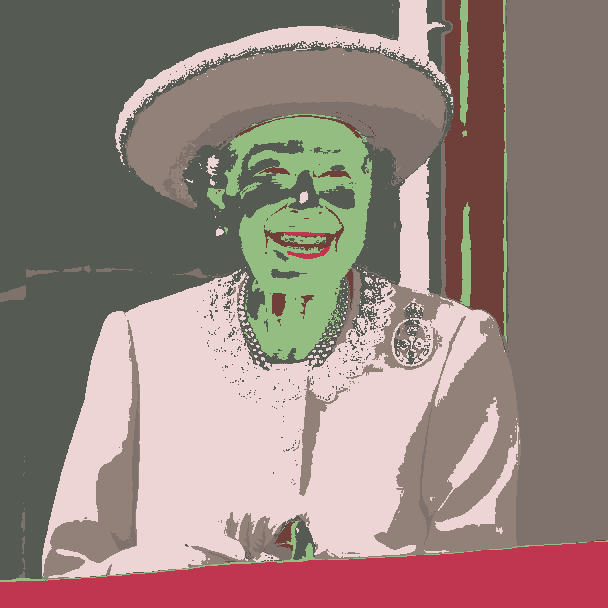
\includegraphics[width=\linewidth]{fig/out/1.2.lab_clustered_edited.png}
        \caption{Shrekified queen}
        \label{fig:1.2.lab_edited}
    \end{subfigure}
    \begin{subfigure}[]{0.3\linewidth}
        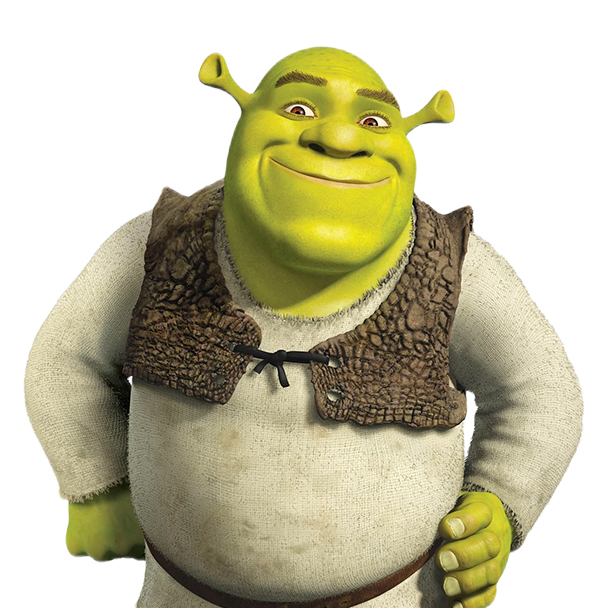
\includegraphics[width=\linewidth]{fig/1.2.shrek.jpg}
        \caption{Actual Shrek}
        \label{fig:1.2.shrek}
    \end{subfigure}
    \caption{Shrek.}
    \label{fig:1.2.edited}
\end{figure}



\section{Color Quantization and lookup tables (LUTs) [3 points]}
In this exercise we are required to compute Lookup Tables (LUT) for mapping the colors of an image to a reduced color palette. A simplified version of the function shown in the previous section [\autoref{fig:1.1.quantization_code}] that does just that is shown below in \autoref{fig:2.code}. Notice how variable \verb|cluster_idx| is the Lookup Table. It contains for each pixel the cluster index to which it belongs to. Variable \verb|cluster_color| instead contains the color of each cluster, useful for finally mapping each pixel to its corresponding color in the reduced palette. The resulting image is computed by substituting each index in the 2D LUT matrix with the corresponding 3-dimensional cluster color.
\begin{figure}[h!]
    \vspace*{-0.2cm}
    \inputminted[firstline=37, frame=lines, framesep=2mm, fontsize=\small ]{matlab}{../src/ex2.m}
    \vspace*{-0.5cm}
    \caption{\small Matlab function computing the LUT of an image}
    \label{fig:2.code}
\end{figure}
Apart from performing color quantization in the HSV space, we can also perform it in the CIELab space. Results are shown in \autoref{fig:2}. We clearly notice how the CIELab color quantization shown in \autoref{fig:2.lab} yields a better result than the HSV one in \autoref{fig:2.hsv}. The clustering quality difference is particularly noticeable in the facial region, as the palette colors better resemble the ones founds in the original image. For computing the grayscale LUT, we simply cluster the image in the CIELab space, and then isolate the grayscale information by taking the first channel L* (luminance). The resulting image is shown in \autoref{fig:2.gray}.

\begin{figure}[h!]
    \begin{subfigure}[]{0.245\linewidth}
        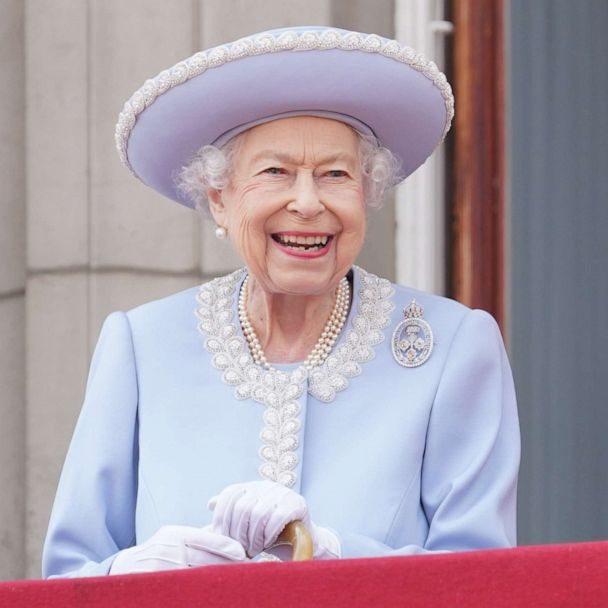
\includegraphics[width=\linewidth]{fig/out/2.img.png}
        \caption{Original image}
        \label{fig:2.img}
    \end{subfigure}
    \begin{subfigure}[]{0.245\linewidth}
        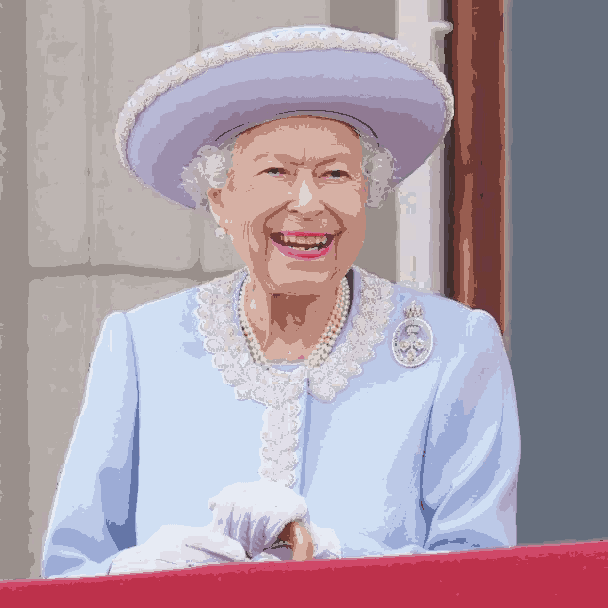
\includegraphics[width=\linewidth]{fig/out/2.hsv.png}
        \caption{HSV color space}
        \label{fig:2.hsv}
    \end{subfigure}
    \begin{subfigure}[]{0.245\linewidth}
        \includegraphics[width=\linewidth]{fig/out/2.lab.png}
        \caption{CIELab color space}
        \label{fig:2.lab}
    \end{subfigure}
    \begin{subfigure}[]{0.245\linewidth}
        \includegraphics[width=\linewidth]{fig/out/2.gray.png}
        \caption{Grayscale-mapped}
        \label{fig:2.gray}
    \end{subfigure}
    \caption{Quantized images with 32 clusters (colors) in different color spaces}
    \label{fig:2}
\end{figure}
\begin{figure}[h!]
    \vspace*{-0.2cm}
    \inputminted[firstline=15, lastline=17, frame=lines, framesep=2mm, fontsize=\small ]{matlab}{../src/ex2.m}
    \vspace*{-0.5cm}
    \caption{Matlab code for computing the grayscale LUT of an image}
    \label{fig:2.gray.code}
\end{figure}


\section{Gaussian and Laplacian Pyramids [4 points]}
The Gaussian pyramid of an image is a sequence of images obtained by repeatedly applying Gaussian blurring and downsampling the original image. The Laplacian pyramid is a sequence of images obtained by subtracting from each image in the Gaussian pyramid the upsampled version of the next image in the Gaussian pyramid. Therefore each layer of the Lapacian pyramid contains just the details of the corresponding layer in the Gaussian pyramid. To reconstruct the original image we simply add each Laplacian layer to its next upsampled pyramid layer.

The Matlab code used to compute the Gaussian and Laplacian pyramids and reconstruct the original image are shown in \autoref{fig:3.code}. The resulting Gaussian and Laplacian pyramids of the image \verb|happy.jpg| are shown in \autoref{fig:3.pyramids}. The reconstructed image is shown in \autoref{fig:3.reconstructed}. 


\begin{figure}[h!]
    \vspace*{-0.2cm}
    \inputminted[firstline=57, frame=lines, framesep=2mm, fontsize=\small ]{matlab}{../src/ex3.m}
    \vspace*{-0.5cm}
    \caption{Matlab functions computing the Gaussian and Laplacian pyramids and reconstructing the original image.}
    \label{fig:3.code}
\end{figure}

\begin{figure}[h!]
    \centering
    \begin{subfigure}[t]{.7\linewidth}
        \begin{subfigure}[t]{\linewidth}
            \includegraphics[height=3.81cm]{fig/out/3.happy_gaussian_pyramid_1.png}
            \includegraphics[height=3.81cm]{fig/out/3.happy_gaussian_pyramid_2.png}
            \includegraphics[height=3.81cm]{fig/out/3.happy_gaussian_pyramid_3.png}
            \includegraphics[height=3.81cm]{fig/out/3.happy_gaussian_pyramid_4.png}
            \includegraphics[height=3.81cm]{fig/out/3.happy_gaussian_pyramid_5.png}
            \caption{Gaussian Pyramid layers}
            \label{fig:3.gaussian_pyramid}
        \end{subfigure}
        \begin{subfigure}[t]{\linewidth}
            \includegraphics[height=3.81cm]{fig/out/3.happy_laplacian_pyramid_1.png}
            \includegraphics[height=3.81cm]{fig/out/3.happy_laplacian_pyramid_2.png}
            \includegraphics[height=3.81cm]{fig/out/3.happy_laplacian_pyramid_3.png}
            \includegraphics[height=3.81cm]{fig/out/3.happy_laplacian_pyramid_4.png}
            \includegraphics[height=3.81cm]{fig/out/3.happy_laplacian_pyramid_5.png}     
            \caption{Laplacian Pyramid layers (brightness artifically increased)}
            \label{fig:3.laplacian_pyramid}
        \end{subfigure}
    \end{subfigure}
    \begin{subfigure}[t]{.15\linewidth}
        \centering
        \begin{subfigure}[t]{\linewidth}
            \centering
            \includegraphics[height=3.81cm]{fig/out/3.happy.png}
            \caption{Original}
            \label{fig:3.original}
        \end{subfigure}
        \begin{subfigure}[t]{\linewidth}
            \centering
            \includegraphics[height=3.81cm]{fig/out/3.happy_reconstructed.png}
            \caption{Reconstructed}
            \label{fig:3.reconstructed}
        \end{subfigure}
    \end{subfigure}
    \caption{Image pyramid decomposition of \texttt{happy.jpg}}
    \label{fig:3.pyramids}
    \vspace*{-0.5cm}
\end{figure}




\section{Hybrid Images [3 points]}

A fun application of Gaussian and Laplacian pyramids is the creation of hybrid images. In essence, the hu-
man visual system is sensitive to high-frequency content of the image at close distances, but the further we move from the image our sensitivity and ability to resolve high-frequency content diminishes, and we better perceive low-spatial frequencies of the image. This can be exploited to create images which combine the high-frequency component of one image with the low-frequency component of another, resulting in an image that changes its appearance depending on the distance from which it is observed.

\begin{figure}[H]
    \centering
    \begin{subfigure}[]{\linewidth}
        \includegraphics[width=.09\linewidth]{fig/out/4.hybrid_sigma(0.5).jpg}
        \includegraphics[width=.09\linewidth]{fig/out/4.hybrid_sigma(1.0).jpg}
        \includegraphics[width=.09\linewidth]{fig/out/4.hybrid_sigma(1.5).jpg}
        \includegraphics[width=.09\linewidth]{fig/out/4.hybrid_sigma(2.0).jpg}
        \includegraphics[width=.09\linewidth]{fig/out/4.hybrid_sigma(2.5).jpg}
        \includegraphics[width=.09\linewidth]{fig/out/4.hybrid_sigma(3.0).jpg}
        \includegraphics[width=.09\linewidth]{fig/out/4.hybrid_sigma(3.5).jpg}
        \includegraphics[width=.09\linewidth]{fig/out/4.hybrid_sigma(4.0).jpg}
        \includegraphics[width=.09\linewidth]{fig/out/4.hybrid_sigma(4.5).jpg}
        \includegraphics[width=.09\linewidth]{fig/out/4.hybrid_sigma(5.0).jpg}
    \end{subfigure}
    \caption{Hybrid images with different $\sigma$ values. Lower-Higher $\sigma$ from left to right.}
    \label{fig:4.hybrids}
\end{figure}

In \autoref{fig:4.hybrids} we present a set of hybrid images created from \texttt{sad.jpg} and \texttt{happy.jpg}. These images have been created by combining the low-frequency component of the first image with the high-frequency component of the second image using low-pass and high-pass filters. Different cut-off frequencies have been used from $\sigma=0.5$ (image at the most left) to $\sigma=5.0$ (image at the most right).

As can be seen, the "sad" component is dominant in the image at the most left while the "happy" smile becomes more and more visible as the cut-off frequency increases. The image at the most right is dominated by the "happy" smile.

Obviously, the effect varies depending on the size of the image on the screen and the viewing distance.


\begin{figure}[H]
    \centering
    \begin{subfigure}[]{.8\linewidth}
        \begin{subfigure}[]{.25\linewidth}
            \includegraphics[width=\linewidth]{fig/out/4.hybrid_sigma(2.5).jpg}
        \end{subfigure}
        \begin{subfigure}[]{.2\linewidth}
            \includegraphics[width=\linewidth]{fig/out/4.hybrid_sigma(2.5).jpg}
        \end{subfigure}
        \begin{subfigure}[]{.16\linewidth}
            \includegraphics[width=\linewidth]{fig/out/4.hybrid_sigma(2.5).jpg}
        \end{subfigure}
        \begin{subfigure}[]{.128\linewidth}
            \includegraphics[width=\linewidth]{fig/out/4.hybrid_sigma(2.5).jpg}
        \end{subfigure}
        \begin{subfigure}[]{.1024\linewidth}
            \includegraphics[width=\linewidth]{fig/out/4.hybrid_sigma(2.5).jpg}
        \end{subfigure}
        \begin{subfigure}[]{.08192\linewidth}
            \includegraphics[width=\linewidth]{fig/out/4.hybrid_sigma(2.5).jpg}
        \end{subfigure}
    \end{subfigure}
    \caption{Showcase of frequency band sensitivity of the human visual system related to the image size.}
    \label{fig:4.showcase}
\end{figure}

\autoref{fig:4.showcase} shows the hybrid image created with $\sigma=2.5$ in different sizes. As the image gets smaller, the "sad" component becomes more and more visible. This is because the high-frequency component of the image is more visible at close distances, while the low-frequency component is more visible at larger distances.

The central image in \autoref{fig:4.showcase} displayed on this report printed on A4 paper, has a width of about 2.2cm. By inspecting the printed image, the "happy" smile is viewed optimally when looking at the image from a distance smaller than about 1.21m. By moving away from the image, the "sad" component becomes more and more visible and it is viewed optimally when looking at the image from a distance of about 1.86m or more.

 
\section{Theory: Hybrid Images [3 points]}
Consider the task of creating a hybrid image from two input images by combining two levels of Laplacian
pyramids. Assume that both images have resolutions $1024 \times 1024$ pixels and the size of the hybrid image
shown on the screen will be $30 \times 30$ centimeters. Additionally, we want the content of one image to be best visible at a distance of 1 meter and the content of the other image to be best visible at a distance of 8 meters. 

From a distance of 1m with 1 visual degree of angle, the width of the visual field is 1.75 cm.
Since the image is 1024 pixels wide and displayed on the screen with a width of 30 cm, the visual field is $\frac{1.75\times 1024}{30} \approx 60$ pixels wide.
The human eye is more sensitive to some frequencies (around 3 cycles/visual degree) so we need to choose the Laplacian levels accordingly.

Each level of the Laplacian pyramid covers a different frequency band: we can say that "roughly" $k$\textsuperscript{th} level contains frequencies $\mu \in (0.5^{k+1},0.5^{k}]$ cycles/pixel.
So:
\begin{align*}
    0.5^k \cdot 60 &\approx 3 \\
    \frac1{2^k} \cdot 60 &\approx 3 \\
    \frac{60}{2^k} &\approx 3 \\
    2^k &\approx 20 \\
    k &\approx \log_2(20) \\
    k &\approx 4.32
\end{align*}
The best visible level of the Laplacian pyramid from a distance of 1m is thus the 4\textsuperscript{th} level.

The same reasoning can be applied to the second image, which has to be best visible from a distance of 8m.
From a distance of 8m with 1 visual degree of angle, the width of the visual field is 13.96 cm.
Since the image is 1024 pixels wide and displayed on the screen with a width of 30 cm, the visual field is $\frac{13.96\times 1024}{30} \approx 476.6$ pixels wide.
As before:
\begin{align*}
    0.5^k \cdot 476.6 &\approx 3 \\
    k &\approx 7.31 \\
\end{align*}
The best visible level of the Laplacian pyramid from a distance of 8m is thus the 7\textsuperscript{th} level.

In conclusion, the chosen levels of the Laplacian pyramid to create a hybrid image that is best visible from a distance of 1m and 8m are 4 and 7 for the first and second images respectively.


\section{Bonus: Create your own Instagram Filter! [10 points]}


In this last section, we present our own Instagram filter. 
The filter is composed of three steps: at first, the colors of the image are clustered into 16 clusters using the k-means algorithm and the colors of the image are replaced with the centroids of the clusters. Then, the edges of the original image are detected using the Canny edge detector and the edges are overlayed on top of the image in black. Finally, the image is slightly saturated to give a more cartoonish look.

\begin{figure}[H]
    \centering
    \begin{subfigure}[t]{.245\linewidth}
        \includegraphics[width=\linewidth]{fig/out/6.img.jpg}
        \caption{Original image}
        \label{fig:6.img}
    \end{subfigure}
    \begin{subfigure}[t]{.245\linewidth}
        \includegraphics[width=\linewidth]{fig/out/6.img_clustered.jpg}
        \caption{Quantized image}
        \label{fig:6.img_clustered}
    \end{subfigure}
    \begin{subfigure}[t]{.245\linewidth}
        \includegraphics[width=\linewidth]{fig/out/6.img_clustered_edges.jpg}
        \caption{Edges of quantized image}
        \label{fig:6.img_clustered_edges}
    \end{subfigure}
    \begin{subfigure}[t]{.245\linewidth}
        \includegraphics[width=\linewidth]{fig/out/6.im_stylized.jpg}
        \caption{Masked and saturated final image}
        \label{fig:6.im_stylized}
    \end{subfigure}
    \caption{Filter steps}
    \label{fig:6.im_filtered_ig}
\end{figure}

\autoref{fig:6.im_filtered_ig} presents the various steps of the filter: the original image (\autoref{fig:6.img}), the image with the colors clustered(\autoref{fig:6.img_clustered}), the edges of the image (\autoref{fig:6.img_clustered_edges}) and the final image with the edges overlayed and saturated (\autoref{fig:6.im_stylized}).

The MATLAB implementation of the filter is shown in \autoref{code:6.ig_filter}.


\begin{figure}[H]
    \vspace*{-0.2cm}
    \inputminted[firstline=17, frame=lines, framesep=2mm, fontsize=\small ]{matlab}{../src/ex6.m}
    \vspace*{-0.5cm}
    \caption{Matlab function applying the \textit{Borderlands 2} filter.}
    \label{code:6.ig_filter}
\end{figure}


\end{document}